\section{Các câu lệnh hợp ngữ}
	\subsection{Sơ đồ chương trình BE-PUM}
	\subsection{Phân tích class}

\newpage
\section{Windows API} \label{sec:wapi_design}

	\subsection{Các thành phần chính của bộ xử lý Windows API} \label{sec:main_classes}

	\begin{figure}[htp]
	\centering
		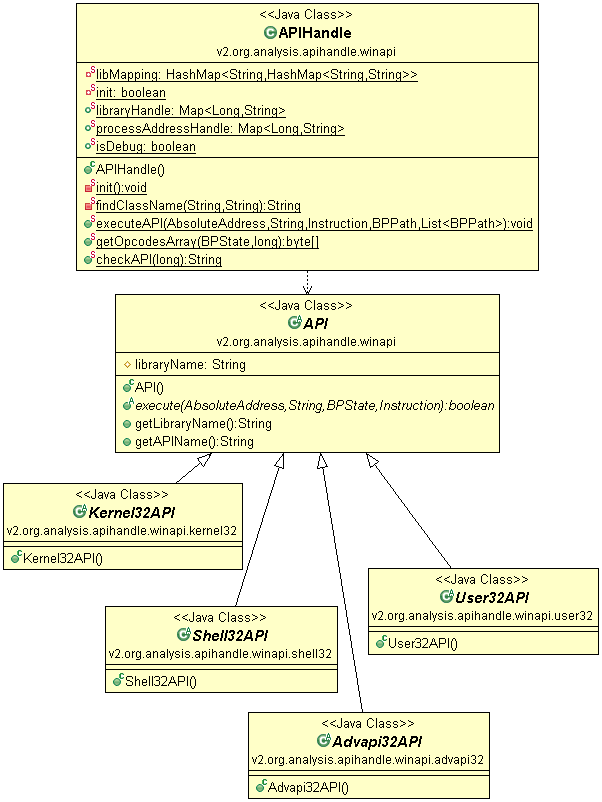
\includegraphics[scale=0.74]{wapi_1_main_classes.png}
		\caption{Kiến trúc chính của bộ xử lý Windows API dành cho BE-PUM}	
		\label{fig:wapi_1_main_classes}		
	\end{figure}

Hình \ref{fig:wapi_1_main_classes} mô tả lược đồ lớp (class) chính được xây dựng cho bộ xử lý Windows API. Trong đó có một class nắm giữ toàn bộ giao tiếp và làm việc giữa hệ thống BE-PUM và các xử lý chính cho từng API đó là class \textit{APIHandle}. Mỗi khi hệ thống BE-PUM cần xử lý một API bất kỳ nào đó, phương thức \textit{executeAPI} của \textit{APIHandle} sẽ được gọi để làm việc.\\

Kiến trúc chính của đề tài được xây dựng dựa trên dạng thức thiết kế adapter hay còn gọi là dạng thiết kế điều hợp. Với adapter là lớp trừu tượng – abstract class: lớp \textit{API}, mỗi bộ thư viện Windows API sẽ được trừu tượng hóa thành từng abstract class mà sẽ kế thừa từ lớp \textit{API} (ví dụ như các lớp \textit{Kernel32API}, \textit{User32API},…). Rồi sau đó, mỗi Windows API sẽ được trừu tượng hóa thành một class, được đặt tên trùng với tên của chính Windows API đó, kèm theo sẽ là việc kế thừa và hiện thực đúng abstract class của bộ thư viện mà Windows API thuộc về.\\

Hình \ref{fig:wapi_2_implemented_classes} ngay sau đây sẽ mô tả ngắn gọn cho việc hiện thực từng Windows API của bộ thư viện dịch vụ nền được chứa trong tập tin \textit{kernel32.dll}.

	\begin{figure}[htp]
	\centering
		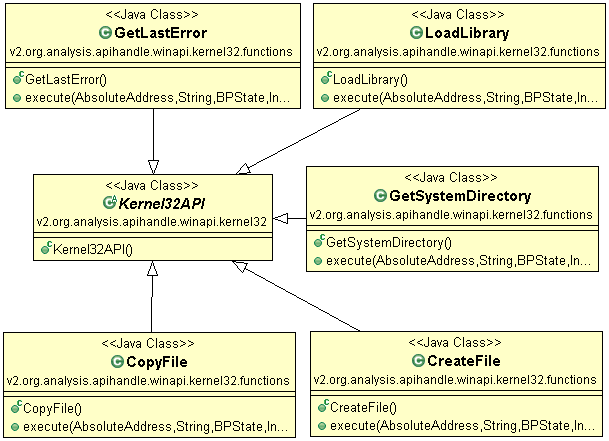
\includegraphics[scale=0.74]{wapi_2_implemented_classes}
		\caption{Mô hình hiện thực một số Windows API trong \textit{kernel32.dll}}	
		\label{fig:wapi_2_implemented_classes}		
	\end{figure}

	\newpage
	\subsection{Những khai báo ánh xạ của bộ xử lý Windows API} \label{sec:mapping}

Ngoài những thành phần chính nêu trên, bộ xử lý Windows API còn có những lớp khác để nắm thông tin ánh xạ giữa hai ngôn ngữ lập trình Java và C thông qua JNA.

	\begin{figure}[H]
	\centering
		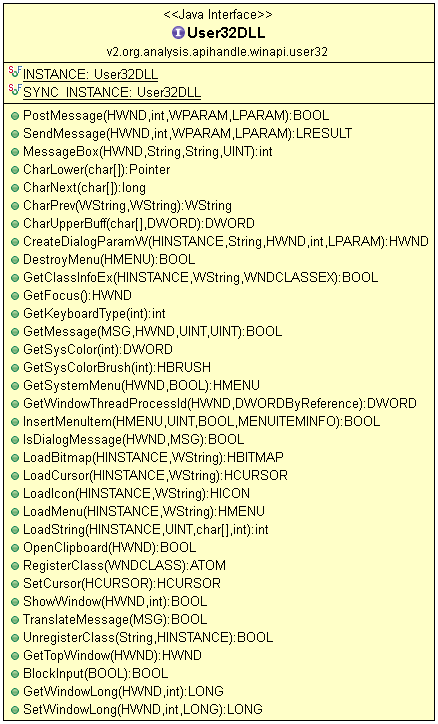
\includegraphics[scale=0.74]{wapi_3_function_map.png}
		\caption{Lớp chứa thông tin ánh xạ những Windows API trong \textit{user32.dll}}	
		\label{fig:wapi_3_function_map}		
	\end{figure}

Trong Hình \ref{fig:wapi_3_function_map} là một mô tả về ánh xạ tên hàm và kiểu dữ liệu đầu vào của bộ thư viện giao diện người dùng được chứa trong tập tin \textit{user32.dll}. Ngoài ra, bộ thư viện JNA có khai báo ánh xạ sẵn một số hàm Windows API cùng những kiểu dữ liệu chính mà Windows API thường dùng, nhờ đó mà những kiểu dữ liệu thông dụng như \textit{HWND, HINSTANCE, LPARAM, DWORD,…} không đòi hỏi lập trình viên phải khai báo và ánh xạ lại.\\

Nhưng không phải tất cả kiểu dữ liệu đề có sẵn, đặc biệt là những kiểu dữ liệu cấu trúc, cần có những trường hợp phải khai báo thêm để ánh xạ và phục vụ cho đề tài này.

	\begin{figure}[H]
	\centering
		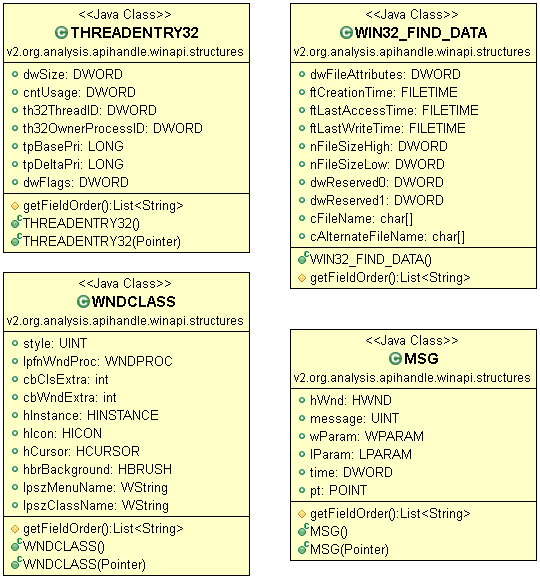
\includegraphics[scale=0.74]{wapi_4_structure}
		\caption{Một số dữ liệu kiểu cấu trúc được xây dựng thêm}	
		\label{fig:wapi_4_structure}		
	\end{figure}

Nội dung của Hình \ref{fig:wapi_4_structure} thể hiện khai báo thêm của một số dữ liệu kiểu cấu trúc dành cho đề tài này. Như đã nói ở Mục \ref{sec:structure}, việc xây dựng này đòi hỏi phải chính xác về kích thước và trình tự các biến được khai báo bên trong struct, để dữ liệu được nạp ra vào chính xác.

	\subsection{Kiến trúc xây dựng và làm việc}

Từ những thành phần đã trình bày ở Mục \ref{sec:main_classes} và Mục \ref{sec:mapping}, kiến trúc của bộ xử lý Windows API sẽ được tổ chức lại cho thống nhất và dễ dàng mở rộng về sau:

	\begin{figure}[H]
	\centering
		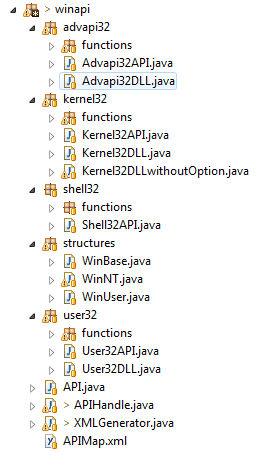
\includegraphics[scale=0.74]{wapi_5_tree}
		\caption{Cây cấu trúc mô tả những thành phần trong bộ xử lý Windows API}	
		\label{fig:wapi_5_tree}		
	\end{figure}

Gói ngoài cùng của bộ xử lý \textit{(winapi)} sẽ nắm:

\begin{itemize}
	\item Khai báo lớp trừu tượng \textit{API}: đặc tả phương thức thực thi dùng chung cho mọi Windows API;

	\item Lớp \textit{APIHandle}: giao tiếp chính giữa bộ xử lý Windows API và hệ thống BE-PUM;

	\item Những gói được đặt tên ứng với từng tên tập tin (không bao gồm phần mở rộng) mà bộ thư viện đó thuộc về. Mỗi gói đó sẽ chứa những thành phần như sau:

	\begin{itemize}
		\item Lớp khai báo trừu tượng cho từng Windows API của bộ thư viện đó (ví dụ như lớp \textit{Kernel32API}), trong đó sẽ nạp vào tên của bộ thư viện hiện tại;

		\item Lớp khai báo ánh xạ thư viện và tên hàm mà hiện bộ thư viện JNA chưa có sẵn (chỉ tồn tại trong trường hợp những Windows API mà đề tài hiện thực chưa có trong bộ thư viện JNA)

		\item Một gói được đặt tên \textit{functions}: dùng để chứa mọi lớp xử lý cho từng Windows API của bộ thư viện hiện tại (ví dụ như hiện tại gói bên ngoài là \textit{kernel32}, những hàm Windows API được xây dựng bên trong sẽ là: \textit{CreateFile, CopyFile, GetLastError…}).
	\end{itemize}

	\item Gói \textit{structures}: chứa những lớp khai báo ánh xạ dữ liệu kiểu cấu trúc mà bộ thư viện JNA chưa có sẵn.

	\item Lớp \textit{XMLGenerator}: có chức năng sinh ra tự động tập tin cấu trúc XML từ tổ chức như trên của bộ xử lý Windows API, mô tả ánh xạ giữa tên của hàm Windows API và tên đầy đủ của lớp sẽ đảm nhận việc xử lý hàm Windows API đó, kèm theo là nó thuộc tập tin thư viện nào. Ví dụ như sau:\\


\lstset{language=HTML}
\begin{lstlisting}
<APIMap>
	<DLL name="advapi32">
		<API funcName="cryptdecrypt" 
className="advapi32.functions.CryptDecrypt"/>
	</DLL>
	<DLL name="kernel32">
		<API funcName="closehandle" 
className="winapi.kernel32.functions.CloseHandle"/>
	</DLL>
</APIMap>
\end{lstlisting}

	\item Tập tin \textit{APIMap.xml}: là nội dung do lớp \textit{XMLGenerator} sinh ra.
\end{itemize}

Nội dung của tập tin \textit{APIMap.xml} được sinh ra dùng để làm chỉ mục cho lớp trung gian \textit{APIHandle} biết được rằng: với thông tin đầu vào là tên của Windows API mà hệ thống BE-PUM yêu cầu, thì lớp nào sẽ xử lý được yêu cầu đó. Sau khi có được tên đầy đủ của lớp xử lý, \textit{APIHandle} sẽ khởi tạo lớp đó với kiểu đối tượng là \textit{API} (do tất cả lớp xử lý đều hiện thực trên lớp này), rồi sau đó gọi phương thức \textit{execute} để đối tượng này xử lý toàn bộ.

	\begin{figure}[H]
	\centering
		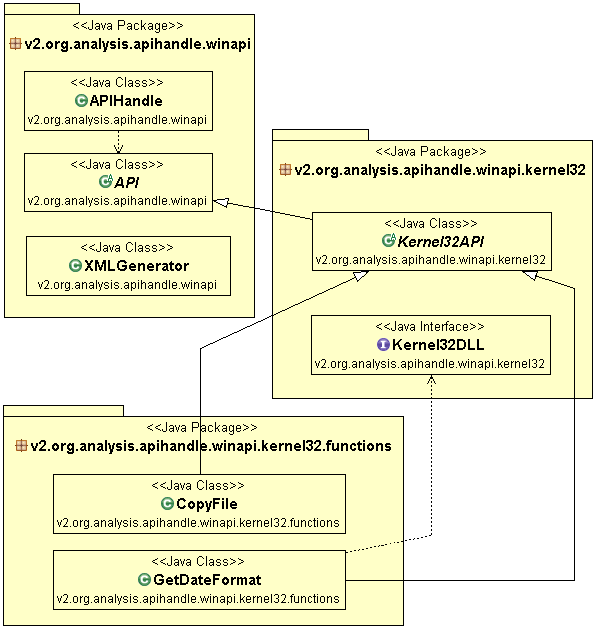
\includegraphics[scale=0.74]{wapi_6_inherited}
		\caption{Giản đồ thể hiện mối liên hệ giữa các thành phần}	
		\label{fig:wapi_6_inherited}		
	\end{figure}


Với việc tổ chức theo cấu trúc này và sinh ra tập tin đánh chỉ mục thì sẽ có được những ưu điểm sau đây:

\begin{itemize}
	\item Dễ dàng quản lý mã nguồn: do Windows API có rất rất nhiều hàm, việc tạo ra mỗi lớp độc lập để xử lý cho từng hàm Windows API sẽ giúp cho mã nguồn được rõ ràng và độc lập cũng như việc sửa chữa sau này được tiện lợi;

	\item Dễ dàng bổ sung: nếu muốn hiện thực thêm một Windows API bất kỳ, ta chỉ việc tạo ra một lớp theo đúng quy định cấu trúc như trên, lớp XMLGenerator sẽ giúp sinh ra nội dung của tập tin APIMap.xml và chỉ đơn giản như vậy là đã tích hợp được một Windows API mới.
\end{itemize}

Nội dung của Hình \ref{fig:wapi_6_inherited} trình bày ví dụ về mối liên hệ mà cấu trúc vừa nêu. Khi hệ thống BE-PUM yêu cầu lớp APIHandle xử lý hàm CopyFile, nó sẽ dùng APIMap.xml để tìm được tên đầy đủ của lớp xử lý được hàm này. Tên ấy được dùng để khai báo khởi tạo động một đối tượng bất kỳ và sau đó ép kiểu về kiểu đối tượng API. Do lớp xử lý được hàm này được hiện thực dựa trên lớp trừu tượng API. Còn với trường hợp nếu là hàm GetDateFormat, thì trong lớp này còn có sử dụng lớp Kernel32DLL do bộ thư viện JNA chưa khai báo sẵn hàm này.

	\subsection{Quản lý môi trường tương tác vật lý}

Do một số Windows API có khả năng làm việc với hệ thống tập tin lưu trữ, dẫn đến khả năng làm ảnh hưởng xấu đến hệ thống do chúng ta đang tập trung vào việc phân tích những phần mềm độc hại cho máy vi tính. Vì vậy ta cần quản lý và ngăn chặn việc đó.\\

Để hiện thực việc đó, một lớp mang tên \textit{Storage} được viết ra để ánh xạ toàn bộ địa chỉ của hệ thống thật vào một vùng lưu trữ đã được quy định. Và rồi mỗi khi một Windows API nào có sử dụng đường dẫn để làm việc, thì cần phải kiểm tra rằng liệu Windows API đó có khả năng ảnh hưởng đến hệ thống hay không, nếu có ta cần ánh xạ sang vùng lưu trữ đã được quản lý để tránh những nguy hại.
